\chapter{Introduction}
	
	3D printing is an manufacturing process where computer models of objects are
	automatically reproduced in a physical form \cite{additivemanufacturing}.
	Figure \ref{fig:gearCube} shows an example of a complex 3D printed object.
	Various 3D printing technologies exist, some of which have gained a number of
	hobbyist-friendly implementations. In this project, a number of improvements
	the popular Makerbot Cupcake CNC 3D printer were made to improve its
	performance.
	
	\begin{figure}
		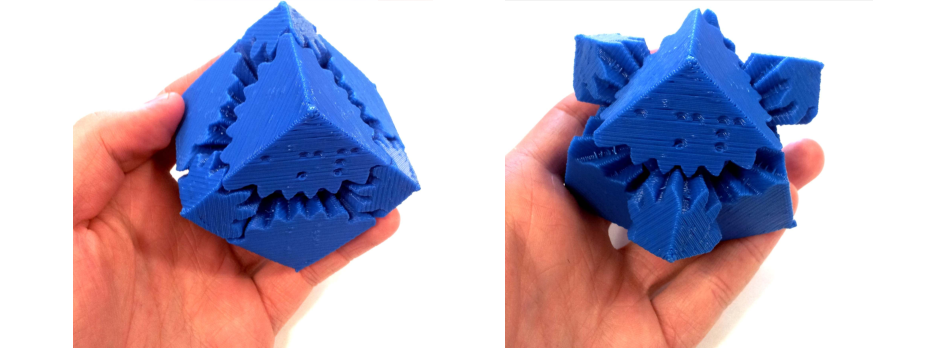
\includegraphics[width=1\textwidth]{diagrams/gearCube.pdf}
		\caption{3D printed `Gear Cube' produced by the printer upgraded in this
		project}
		\label{fig:gearCube}
	\end{figure}
	
	In this chapter the applications of 3D printing are examined followed by an
	introduction to the Makerbot and the improvements made by this project.
	
	\section{Applications}
		
		3D printing technologies allow complex objects, including complete
		mechanisms, to be easily manufactured based on digitized designs in one go
		with a single piece of equipment. Various materials are used including
		metal, various plastics, resins and even sugar \cite{candyfab}.
		
		Rapid prototyping is an obvious application where the flexibility to quickly
		manufacture a wide range of objects extremely valuable. For example, Boeing
		are using 3D printing to reduce the tooling cost and speed up prototyping
		its aeroplanes \cite{boeing3dprint}.
		
		Because there is no tooling cost associated with changing a design, custom
		manufacturing is also possible. This has applications both for personalised
		goods and more recently in the manufacture of bespoke medical implants
		\cite{jaw}.
		
		The cost of entry-level 3D printers has recently become much lower with DIY
		devices such as the RepRap costing between \$300 and \$620 to build
		\cite{costsdown,reprap}. This has helped grow communities such as
		Thingiverse where people share their designs for printable objects with the
		goal of making physical things as easily accessible as any other digital
		media \cite{thingiverse}.
	
	\section{Makerbot}
		
		\label{sec:makerbot_basics}
		
		The Makerbot (figure \ref{fig:makerbotOrig}) is an open source, DIY 3D
		printer which can produce plastic objects up to
		$10\cm\times10\cm\times13\cm$ in size.  It consists of a moving platform
		onto which which an `extruder' melts plastic filament and deposits a thin
		strand of plastic (figure \ref{fig:printerBasics}). Objects are produced by
		moving the platform underneath the extruder and to form layers of plastic
		which are stacked one on top of each other until the complete shape is
		formed. Figure \ref{fig:slicing} shows how a cone (A) might be sliced into
		layers (B) and how each layer might be printed (C).
	
		\begin{figure}
			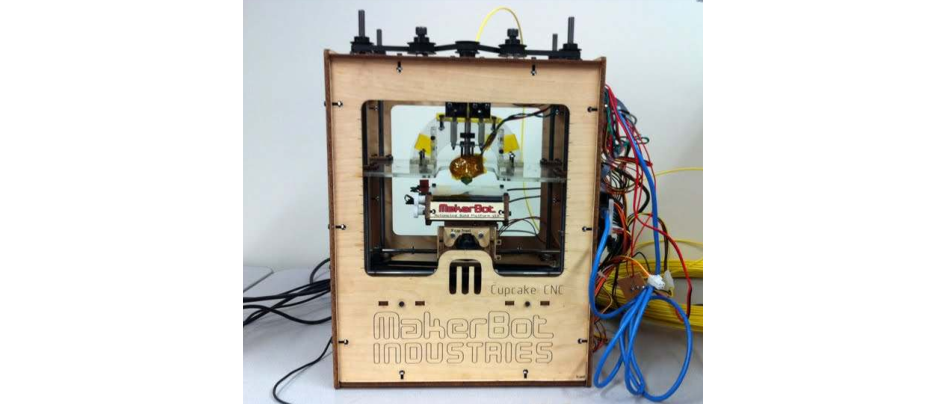
\includegraphics[width=1\textwidth]{diagrams/makerbotOrig.pdf}
			\caption{Unmodified Makerbot Cupcake CNC (photo by Rayshobby
			         \cite{rayshobby})}
			\label{fig:makerbotOrig}
		\end{figure}
	
		\begin{figure}
			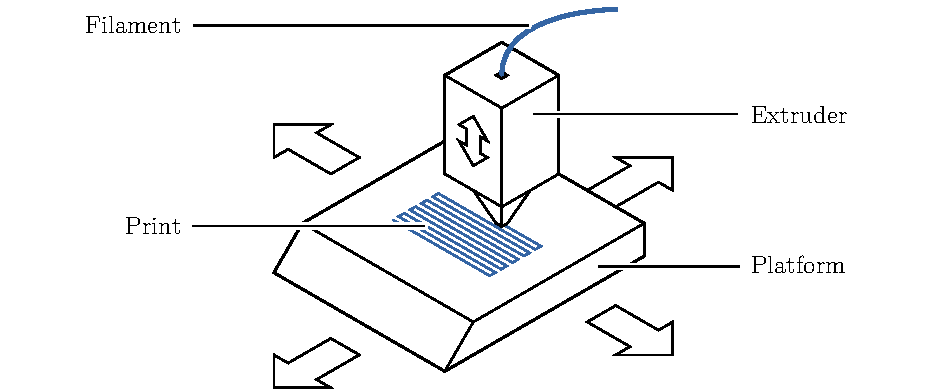
\includegraphics[width=1\textwidth]{diagrams/printerBasics.pdf}
			\caption{Makerbot key components}
			\label{fig:printerBasics}
		\end{figure}
		
		\begin{figure}
			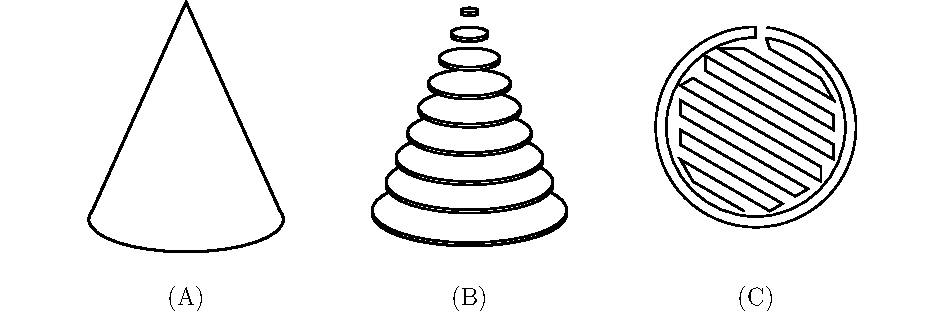
\includegraphics[width=1\textwidth]{diagrams/slicing.pdf}
			\caption{Slicing a 3D model into layers to be printed}
			\label{fig:slicing}
		\end{figure}
		
		Software running on a computer handles the process of slicing a 3D model and
		generating the list of movements required to print it out.  A simple
		microcontroller on the Makerbot receives this list of instructions and
		generates the carefully timed electronic signals needed to drive the
		printer's components.
		
	\section{Project Motivation and Goals}
		
		\label{sec:aims}
		
		The Makerbot, while a very capable machine, has many limitations in its
		hardware, electronics and firmware. In this project the control electronics
		and microcontroller are the primary area for improvement. The existing
		system has trouble with complex designs where dense sequences of
		instructions exceed the microcontroller's limited resources and slow serial
		interface. The electronics are also a complicated configuration of several
		circuit boards using clunky mechanical relays.  Finally, the printer does
		not have sensors to indicate the positions of the platform and extruder
		requiring the platform to be carefully positioned before prints. This is a
		time consuming and error prone task which also means that the printer can't
		detect mechanical errors during printing.
		
		In this project, each of these three complaints are addressed by the
		following primary project goals:
		\begin{description}
			
			\item[Simplify control electronics] Produce a single board which contains
			all required components using only reliable solid-state parts.
			
			\item[Improve performance] Upgrade to a more powerful microcontroller and
			develop new firmware to exploit the resulting improvements in speed and
			communications capabilities.
			
			\item[Add sensors for platform and extruder movements] End-stop sensors at
			the end of each axis of movement will be added to allow the system to
			position itself.
			
		\end{description}
	
	\section{Report Outline}
		
		This report first discusses the background of the project covering 3D
		printing and the technologies selected for the project. In chapter
		\ref{sec:design} the design of system is proposed followed by details of the
		implementation in chapter \ref{sec:implementation}. Chapter
		\ref{sec:testing} describes how the system was tested and evaluates the new
		system's performance. Finally, chapter \ref{sec:conclusions} concludes the
		report and describes opportunities for future work following on from the
		project.
